\documentclass[11pt,a4paper]{article}
\usepackage[top=2cm,bottom=2cm,left=2cm,right=2cm]{geometry}
% \voffset=-2.8cm
% \hoffset=-1.6cm
% \textwidth=14.5cm
% \textheight=24.5cm
\usepackage{amsmath}
\usepackage{amsfonts}
\usepackage{amssymb}
%\usepackage{subfig}
\usepackage{epsfig}
\usepackage{hyperref}
%\usepackage[utf8]{inputenc}
%\usepackage{mathtools}
\usepackage[caption=false]{subfig}
\usepackage{soul,xcolor}
\usepackage{float}
\usepackage{graphicx}
\usepackage{setspace}
\usepackage{mathrsfs}
\usepackage{algorithm}
% \usepackage{algorithmic}
\usepackage{algpseudocode}

\hypersetup{
    colorlinks= true,
    linkcolor= blue,
    filecolor=magenta,      
    urlcolor= blue,
    citecolor = red,
    pdftitle={Overleaf Example},
    pdfpagemode=FullScreen,
    }
    
%---------------------breakable algo--------------------------
\makeatletter
\newenvironment{breakablealgorithm}
  {% \begin{breakablealgorithm}
   \begin{center}
     \refstepcounter{algorithm}% New algorithm
     \hrule height.8pt depth0pt \kern2pt% \@fs@pre for \@fs@ruled
     \renewcommand{\caption}[2][\relax]{% Make a new \caption
       {\raggedright\textbf{\ALG@name~\thealgorithm} ##2\par}%
       \ifx\relax##1\relax % #1 is \relax
         \addcontentsline{loa}{algorithm}{\protect\numberline{\thealgorithm}##2}%
       \else % #1 is not \relax
         \addcontentsline{loa}{algorithm}{\protect\numberline{\thealgorithm}##1}%
       \fi
       \kern2pt\hrule\kern2pt
     }
  }{% \end{breakablealgorithm}
     \kern2pt\hrule\relax% \@fs@post for \@fs@ruled
   \end{center}
  }
\makeatother


%\vspace*{-2cm}
%%%%%%%%%%%%%%%%%%%%%%%%%%%%%%%%%%%%%%%%%%%%%%%%%%%%%%%%%%%%%%%%%%%
\begin{document}
%%%%%%%%%%%%%%%%%%%%%%%%%%%%%%%%%%%%%%%%%%%%%%%%%%%%%%%%%%%%%%%%%%%
\thispagestyle{empty}
\vspace*{0.6cm}
\begin{center}
 
\includegraphics[height=3.5cm,angle=0]{Logo-IITD.jpg}\\
\textbf{Dept of Physics, IIT Delhi}
\end{center}

\vspace*{0.8cm}
\begin{center}
\textbf{Course Code : PYD411}\\
\textbf{Academic Year : 2021 - 2022,\, Semester - II}\\
\end{center}

\vspace*{0.8cm}
\begin{center}
\textbf{\LARGE{Design and characterization of arrays of optical tweezers for single atom trapping}}\\
\end{center}

\vspace*{0.8cm}
\begin{center}
\textbf{\Large{Mayand Dangi}}\\
\end{center}

\vspace*{0.8cm}
\begin{center}
\textbf{\Large{Adviser: Prof. Bodhaditya Santra}}\\
% \textbf{\Large{\hspace*{2.1cm} Prof. Firstname Middlename Lastname}}\\
\end{center}

\vspace*{1.5cm}
\noindent
\textbf{Abstract}: In this project, we are attempting to design optical tweezers capable of capturing a single neutral atom for use in quantum computing. In order to accomplish this goal, a liquid-crystal spatial light modulator is utilised, and a required phase is retrieved using the Gerchberg-Saxton algorithm. We have developed the optical setup and demonstrated the optical tweezers for capturing and transporting the atoms. The next move is to do modification for flicker free movement of optical tweezers.


\vspace*{1cm}

\begin{figure}[H]
\centering

\includegraphics[width=\textwidth]{img/WhatsApp Image 2022-09-29 at 16.47.25.jpeg}
\label{fig:img_target}
% \caption{(a) Source intensity distribution, (b)Target intensity distribution}
\end{figure}
% \begin{flushleft}
% Signature of the student: ................ \\ 
% % \vspace*{0.5cm}
% % Signature of student 2: ................
% \end{flushleft}

% \vspace*{-1.35cm}

% \begin{flushright}
% Signature of the adviser: ................ 
% \end{flushright}
%
% (Please sign in the .... part, if working alone, should be
% ``Signature of the student''. In such case comment out 
% the extra line with \% in front. 
% Also collect signature from your mentor)



%%%%%%%%%%%%%%%%%%%%%%%%%%%%%%%%%%%%%%%%%%%%%%%%%%%%%%%%%%%%%%%%%%%%%%%%%%
\newpage
\thispagestyle{empty}
.
\newpage
% DO NOT TOUCH THIS PART. THIS WILL MAKE SURE THAT
%THE SECOND PAGE, AFTER THE TITLE PAGE SHOULD REMAIN EMPTY
\clearpage
\setcounter{page}{1}
%%%%%%%%%%%%%%%%%%%%%%%%%%%%%%%%%%%%%%%%%%%%%%%%%%%%%%%%%%%%
%%%%%%%%%%%%%%%%%%%%%%%%%%%%%%%%%%%%%%%%%%%%%%%%%%%%%%%%%%%%
\section{Introduction} 
\label{sec:intro}
\onehalfspacing
\noindent
In the famous paper of Richard Feynman, namely "Simulating Physics with Computer", he pointed out that it is impossible to simulate quantum mechanical systems with classical computers due to their complexity \cite{feynman1982simulating}. He also stated that utilizing these complexities of quantum systems using a quantum computer can have a broad revolutionary impact on many challenging problems. According to the DiVincenzo criteria, qubit is one of the necessary criteria for building a quantum computer \cite{divincenzo2000physical}. Extensive research is going on building a quantum computer with different types of qubits such as neutral atoms, ions, superconducting Josephson junctions and optomechanical resonators.

% \subsection{Neutral Atom Qubit}
Among the numerous categories investigated, arrays of single neutral atoms seem to be a very robust and promising technology \cite{saffman2016quantum}. Its long coherence time and high scalability gave it a distinct edge over other qubits, while achieving high gate fidelity on neutral atoms remain a challenge \cite{xia2015randomized}. In a neutral atom qubit, any two states out of many available states can be used for a qubit; however, for a long coherence time, two hyperfine states in the ground state are preferred as a qubit. The realization that optical tweezers can confine neutral atoms inspired the notion of employing them as qubits.  

% \subsection{Optical Traps}
Optical tweezers are a powerful technique for holding and moving atoms that utilizes the electric dipole interaction force to manipulate quantum objects' external degrees of freedom \cite{samoylenko2020single, nogrette2014single, Lee:16}. Optical tweezers capture and isolate a single atom from a precooled ensemble of atoms without inducing optical transitions, preserving the atom's current state. Optical tweezers are considered a versatile tool that can be achieved using microlens arrays \cite{schlosser2011scalable}, diffractive optical elements, optical standing waves \cite{dammann1971high}, spatial light modulators (SLM) \cite{nogrette2014single} and many more. Holographically generated arrays of tightly focused optical tweezers using SLM are typical and more flexible ways of designing optical tweezers.


% Optical dipole trapping is a simple and powerful technique for holding and steering atoms
% in space [36, 37, 38, 39, 40, 41, 42]. This technique, recently developed to far off-resonant optical trapping (FORT), utilizes the electric dipole interaction force exerted by light to manipulate the external degrees of freedom of quantum objects. From a pre-cooled atom ensemble, focused laser beams can capture and isolate single atoms without inducing optical transitions, so their internal states are well preserved in the electronic ground state up to several seconds, which makes the optically trapped single atoms a promising candidate for storing and processing quantum information. Currently there is a strong interest in using the FORT in engineering scalable quantum platforms [8], [44]-[52], because the manipulation of N single atoms in a synthetic structure of a few µm size is a crucial necessity for the study of quantum computation, quantum simulation, and quantum many-body physics [53]-[56]. Optical dipole microtraps and optical lattices [56] are the well-known tools for atom arrays. In the context of the manipulation and control of individual atoms in an array, optical microtraps are considered to be a versatile tool, having many control parameters. The optical microtraps have been achieved by various methods, including micro lens arrays [57], diffractive optical elements such as Dammann grating [58], spatial light modulators (SLM) [8], [45]-[46], optical standing waves [50], and dynamic light deflectors [45]. With these methods, adiabatic transport
% of atoms in one and two dimensions [47]-[48], atom sorting with a cross junction [50], collisional blockade mechanism [52], controlled collisions for near-deterministic atom loading [59], atom array rotations [46], and single-qubit gate arrays [53] have been demonstrated. These impressive achievements are currently being geared towards a deterministically-loaded high-dimensional arbitrary architecture of N single atoms in which the the internal and external degrees of freedom of the atoms are freely controllable.
% Holographic methods of using a programmable SLM in the Fourier domain have been a
% work horse in the construction and manipulation of various forms of two-dimensional (2D)
% microtrap arrays [8]. The SLM phase pattern generation for Ntr ∼ 2N optical microtraps is
% often performed with iterative Fourier transform algorithms (IFTA).

% % Neutral atom arrays in two- or three-dimensional space may
% % play an important role in quantum information processing
% % (QIP), because of their scalability to a massive number of
% % qubits [1–6]. Currently, arrays of several hundred atoms have
% % been implemented with optically addressable spacings of a
% % few μm [7,8], and this number is expected to increase to a few
% % thousand as laser power permits. These atoms are confined
% % by an array of optical-dipole traps made through various
% % methods including holographic devices [9], diffractive optical
% % elements [10,11], microlens arrays [12], and optical lattices
% % [13]. Ultimately, neutral-atom platforms for QIP may require
% % (i) a significant number of atoms, (ii) a high-dimensional
% % architecture, preferably with an arbitrary lattice geometry,
% % (iii) single-atom loading per site, and (iv) the ability to
% % be individually addressable. However, no existing method
% % satisfies all these requirements. For example, optical lattices
% % can provide a large number of atoms singly loaded per site
% % through theMott insulator transition [13], but they have rather
% % limited geometries and often lack individual addressability;
% % other methods have advantages of arbitrary configurations and
% % site addressability but fail the single-atom


% brief about neutral atom qubit and its importance and benifits

% \subsection{Optical Tweezers}
% trapping of atom and ways to do it\\    


% Trapped neutral atoms have intensively studied as physical implementation of qubits for quantum information processing, along with photons [1], trapped ions [2, 3, 4], and superconductors [5, 6]. As a qubit, a neutral atom, as well as a trapped ion, has a clear advantage that it has a well-defined set of quantum states with sharp linewidth, which makes it a well defined qubit with long coherence time. Besides, the history of controlling atoms, or optical spectroscopy, with many kinds of modulated lights makes it more accessible. Also, neutral atom qubits have high scalability [7], in which they are more favorable than trapped ions, as their trap geometries are easily created by a range of light modulation techniques [8]. On the other hand, achieving high gate fidelity on neutral atoms for quantum computing still remains as a challenge yet. Any two states can be used for a qubit in neutral atoms among many states that have variety of physical characteristics such as linewidth and dipole moments. For long coherence time of qubits, any two hyperfine states in the ground state are favored as a qubit.

In this project, we aim to create optical tweezers for trapping the neutral atoms and then implement the algorithm to generate the array of the trapped atom using dynamic holography. Many research groups have attempted various methods to construct arrays of atomic traps that can hold a single atom or a collection of atoms. The approaches utilized range from the multiple dipole trap beams to the creation of optical lattices and arrays of microtraps using fixed optics. Since the probability of an atom getting trapped in an array is 0.5, the probability of getting a perfect array of the atom is not possible. The inflexibility of these methods in terms of the arrangement of atoms is one of the significant problems. Therefore, we have opted to use the SLM for creating optical tweezers, enabling us to apply dynamic holography and reorganize atoms.


% For literature review of single atom trapping and design of optical tweezers using SLM we have refer to "Single-atom trapping in holographic 2D arrays of microtraps with arbitrary geometries." of Antonie's group\cite{lahaye2013single} and  "Formation and Control of Rydberg Atom Arrays for Quantum Information Processing"\cite{lee2019formation} of Jaewook Ahn's group. We have also refered "Single atom movement with dynamic holographic
% optical tweezers"\cite{samoylenko2020single} and "Design strategies for optimizing holographic optical tweezers setups"\cite{martin2007design}.
% Write in a elucidate way 
% your motivation for considering this specific topic / problem. Also mention / discuss observations / results in this area from previous works / studies / analyses, etc (known as the literature survey).. For example, central force problem is a key area of classical mechanics for which one can consider some standard textbook like the one written by Goldstein.

%For journal you should give name of the article, name 
% of author(s), year of publication, volume, number
% and pages


% Here you need to add references to support your literature survey.
% While referencing remember for books you need to
% provide name of the book, name of author(s), publisher,
% date of publication, pages (if known) and ISBN number.
% For journal you should give name of the article, name 
% of author(s), year of publication, volume, number
% and pages. For reports you can also follow the same.
% Please maintain referencing in proper order, i.e., Ref.[1]
% should come before Ref.[2] and not after Ref.[2] or later, so be careful. Use the option cite\{refname\} (a refname is what
% written inside a backslash sign bibitem\{name\}) with a ``backslash sign" before ``cite'' (without any space) to call a reference.
% Example of correct reference in order: Classical mechanics book by Goldstein \cite{Goldstein:2001} / Famous works of Einstein \cite{Einstein:1916vd,Einstein:1935tc}
% and Dirac \cite{Dirac:1948um} / See IIT Delhi physics \cite{iitd:web}
% (if you need to refer a web link), etc.
% Example of wrong order in referencing: Famous works\footnote[1]{You should read these papers.} (example of putting needed but not-directly connected information in footnote) of Einstein \cite{Einstein:1935tc,Einstein:1916vd}.

%%%%%%%%%%%%%%%%%%%%%%%%%%%%%%%%%%%%%%%%%%%%%%%%%%%%%%%%%%%%
%%%%%%%%%%%%%%%%%%%%%%%%%%%%%%%%%%%%%%%%%%%%%%%%%%%%%%%%%%%%
\section{Methodology}
% \section{Design of optical tweezers}
Single atoms held in an array of optical tweezers are necessary for quantum simulation and quantum information processing with Rydberg atoms \cite{saffman2016quantum}. Multiple approaches have been taken to create arrays of atomic traps, of which the use of SLM to create arrays of optical tweezers sounds promising owing to its advantage over other approaches. Optical tweezers made by fixed optics lack flexibility in arrangement. At the same time, holographic arrays have the relative ease of creating arbitrary two-dimensional patterns of optical tweezers and give the flexibility to reconfigure the array \cite{samoylenko2020single}. In our project, we use this technique to design an array of optical tweezers.

\subsection{Optical Setup}
\label{sec2:Optical Setup}
Figure \ref{fig:optical_setup} describes the preliminary experimental setup for generating and characterizing optical tweezers. For the experiment presented in this report, we have used a 632nm diode laser as a light source and Holoeye Pluto Spatial Light Modulator. In the original experiment, a custom-designed external cavity diode laser of 976nm will be used.

In the setup, a collimated gaussian beam with a uniform spatial phase and real amplitude $A_{laser}(x,y) = |A_{laser}(x,y)|$ from the laser falls on the polarizing beam splitting(PBS) cube to have a clean polarization of the beam. Then the beam passes through Beam Expander to ensure complete illumination of the surface of the SLM, and the complex amplitude of the incident beam is given by $A_{in}(x,y)$ \cite{phdthesis1}. Let's assume SLM to be the rectangular aperture of size $L_x \times L_y$ and modulate the phase by $\phi(x,y)$. Then modulated beam immediately after the SLM is given by
\begin{equation}
    A_{SLM} = A_{in}(x,y)\text{rect}(\frac{x}{2L_x},\frac{y}{2L_y})e^{i\phi(x,y)}.
    \label{eq:1}
\end{equation}
The beam is now passed through the iris having an opening of radius $r$. Afterwards, it is finally focused by the lens of focal length f in the focal plane, in the preliminary optics setup. The amplitude distribution at the focal plane is the same as the amplitude of the targeted intensity distribution given by,
\begin{equation}
    \Tilde{A}_f(\Tilde{x},\Tilde{y}) = \mathscr{F}[A_{SLM}(x,y)\text{circ}(r)].
    \label{eq:2}
\end{equation}

The optics setup shown in figure \ref{fig:optical_setup_real} will be used in actual experiment. The beam after getting modulated by SLM, is reflected from a dichroic mirror having a good reflectivity at 976nm wavelength and transmissivity at 852 nm and will be focused by microscope objective inside the glass cell. The focused tweezers array is imaged by a CCD camera. After loading, the atoms' fluorescence is collected by the same objective lens and transmitted through the dichroic mirror to image it on the CMOS camera. The intensity pattern obtained on the screen of the CMOS camera will be used to determine the position of trapped atoms. The position of the trapped atom is one of the input parameters for the path planning algorithm to ensure that the trapped array configuration is defect-free.\\


\begin{figure}[H]
\centering
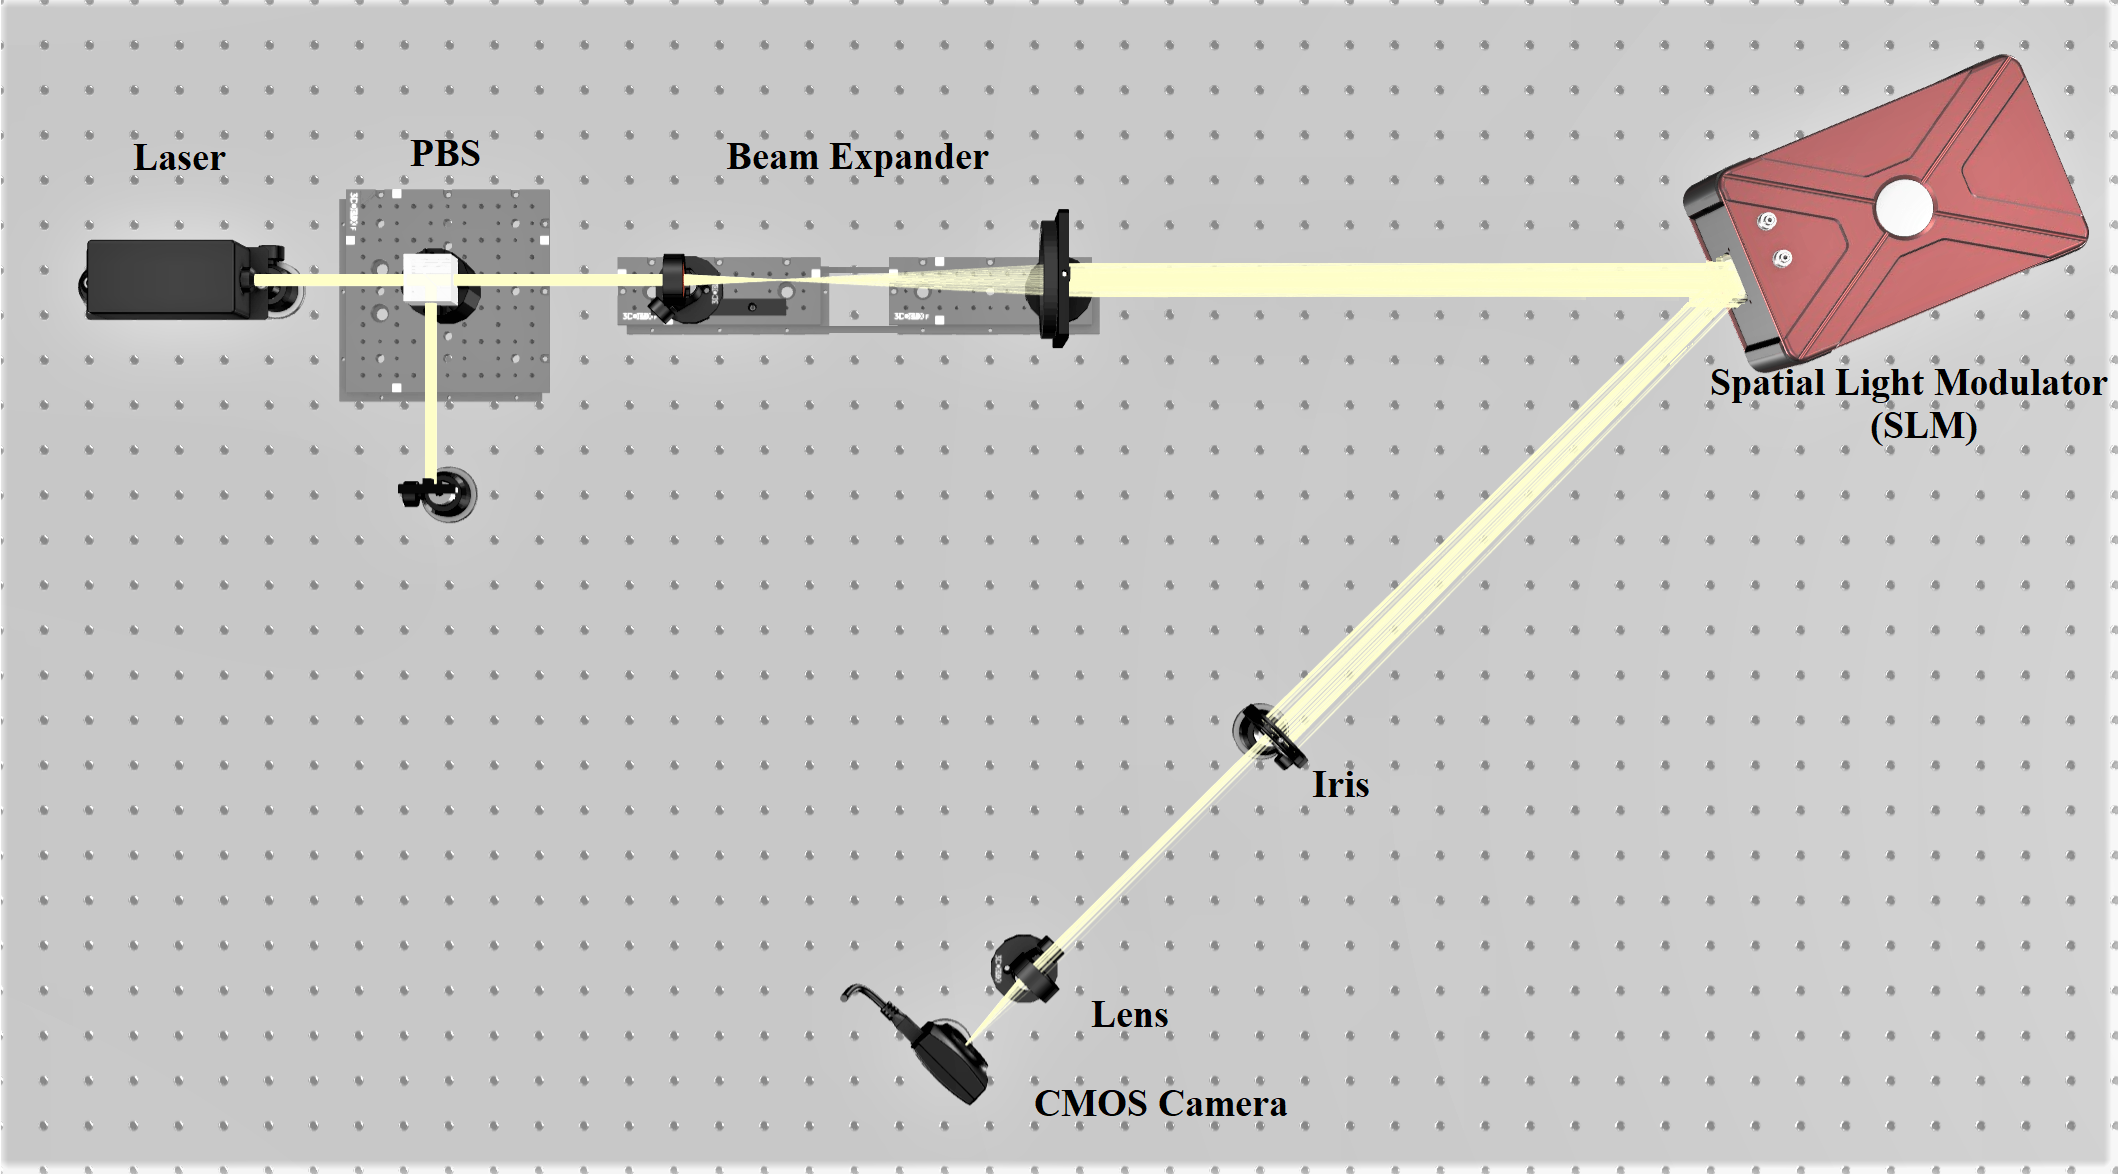
\includegraphics[width=0.8\textwidth]{img/optical_setup.jpg}
\onehalfspacing
\caption{Preliminary Optics setup for the SLM}
\label{fig:optical_setup}
\end{figure}

\begin{figure}[H]
\centering
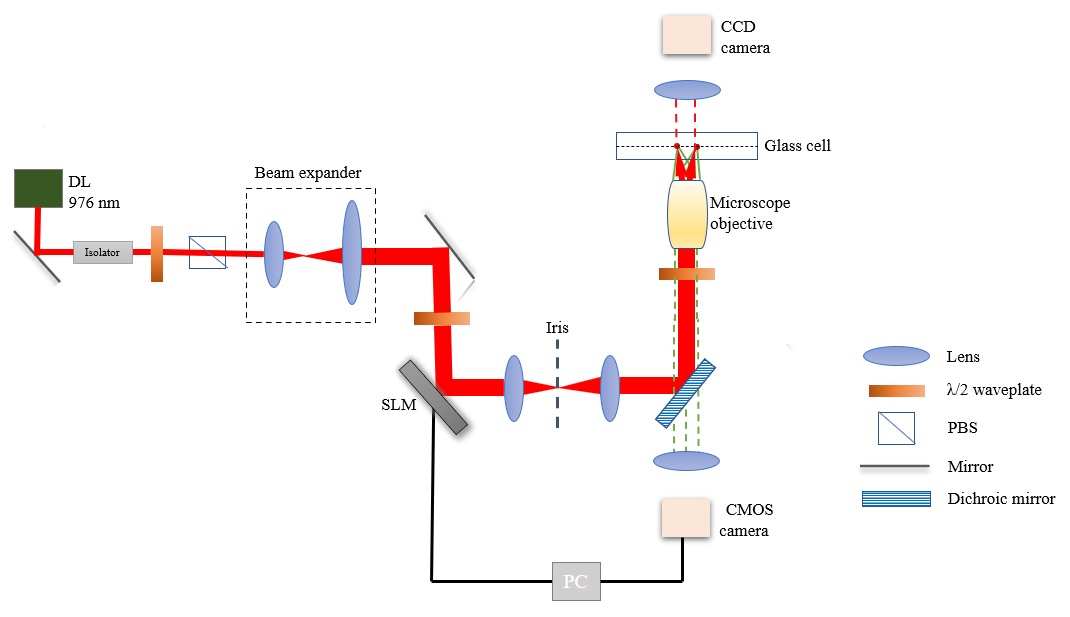
\includegraphics[width=\textwidth]{img/expsetup - Copy.png}
\onehalfspacing
\caption{Proposed Optics setup for trapping atom using optical tweezers}
\label{fig:optical_setup_real}
\end{figure}
\vspace{1em}
\begin{figure}[H]
\centering
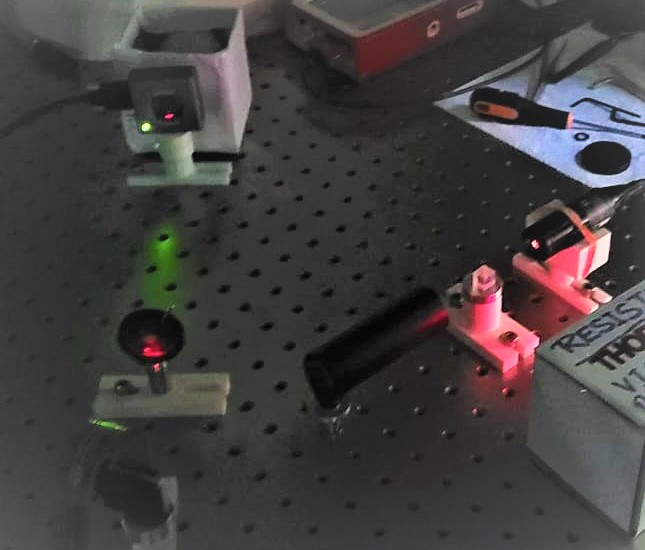
\includegraphics[width=0.75\textwidth]{img/setup on optical table 2.jpeg}
\caption{Optical setup for generating an array of optical tweezers}
\label{fig:optical_setup_lab}
\end{figure}


\subsection{Design of optical tweezers}
From the equation \ref{eq:2} of the previous section, we can see that fourier transform result strongly depends on the $\phi(x,y)$ term. Since we are using phase-only SLM in the experiment. Thus, it becomes crucial to retrieve the phase corresponding to the target intensity distribution of array of optical tweezers.

\subsubsection{Phase-mask generation}
We are using Gerchberg–Saxton(GS) algorithm for the generation phase mask that has to be imprinted on SLM \cite{gerchberg1972practical}. This algorithm was initially used in electron beam microscopy to retrieve phase information from the intensity distribution, which is also known as Error-reduction algorithm \cite{khare2015fourier}. It has now become a usual choice as a phase retrieval algorithm for beam shaping and optical information processing.

The GS algorithm uses the iterative virtual propagation of the light field between the SLM's plane and the lens' focal plane, intending to converge on an appropriate phase to produce a targeted intensity distribution. The algorithm for the GS algorithm is proposed below:

\begin{breakablealgorithm}
\caption{: Gerchberg–Saxton(GS) algorithm}\label{alg:GS}
\algrenewcommand\algorithmicrequire{\textbf{Input:}}
\algrenewcommand\algorithmicensure{\textbf{Output:}}
    \begin{algorithmic}
        \Require  $A_{source}$,  $A_{target}$, $\phi_{r}$, iter
        \Ensure $\phi_{r}$ 
        \State A $\leftarrow$ $exp(i\phi_r)$
        \State $i\leftarrow 0$
        \While{$i<$iter}
            \State $B \leftarrow abs(A_{source})*exp(i*angle(A))$
            \State $C \leftarrow FFT[B]$
            \State $D \leftarrow abs(A_{target})*exp(i*angle(C))$
            \State $A \leftarrow IFFT[D]$
        \EndWhile
        \State $\phi_r \leftarrow angle(A)$
        \State \Return $\phi_r$
\end{algorithmic}
\end{breakablealgorithm}

To determine the adequate phase pattern corresponding to the targeted intensity distribution, we have to numerically implement the above described GS algorithm. For this we have discretized the field in $N_x \times N_y$ matrix in SLM plane with spacing of one cell as $\triangle_x \times \triangle_y$. Thus, we can write discrete complex amplitude in the SLM field as
\begin{eqnarray}
    \label{eq:discrete_A_slm}
    A_{SLM}(m\triangle_x,n\triangle_y) = A_{in}(m \triangle_x, n \triangle_y)e^{i\phi_{mn}},
\end{eqnarray}
\begin{equation}
    A_{SLM}(x,y) = \sum_{m=0}^{N_x-1}\sum_{n=0}^{N_y-1} \delta(x-m \triangle_x) \delta(y-n \triangle_y) A_{in}(m \triangle_x, n \triangle_y)e^{i\phi_{mn}},
\end{equation}
where, $A_{in}(\alpha \triangle_x, \beta \triangle_y)$ is the incident light field on the SLM which is same as the $A_{source}$ described in algorithm \ref{alg:GS} and $\phi_{\alpha \beta}$ is the phase delay obtained using the GS algorithm corresponding to the pixel $\alpha \beta$.
The field in focal plane of the lens is given by \cite{khare2015fourier, nla.cat-vn592477},
\begin{eqnarray}
    \Tilde{A}_f(u \Tilde{\triangle}_x, v \Tilde{\triangle}_x) =  \text{DFT}[A_{SLM}(m\triangle_x,n\triangle_y)],
\end{eqnarray}
\begin{equation}
\label{ref:eq_FocalAmp}
    \Tilde{A}_f(u \Tilde{\triangle}_x, v \Tilde{\triangle}_x) = \sum_{m=0}^{N_x-1}\sum_{n=0}^{N_y-1} A_{in}(m \triangle_x, n \triangle_y)e^{i\phi_{mn}}e^{-2\pi i(mu/N_x + nv/N_y)},
\end{equation}
where, 
\begin{equation}
\label{ref:eq_focaltoslm}
    \Tilde{\triangle}_x=\frac{\lambda f}{L_x}\text{  and  } \Tilde{\triangle}_y=\frac{\lambda f}{L_y}.
\end{equation}
\begin{equation}
\label{ref:eq_slmtofocal}
    \Tilde{L}_x=\frac{\lambda f}{\triangle_x}\text{  and  } \Tilde{L}_y=\frac{\lambda f}{\triangle_y}.
\end{equation}
The equation \ref{ref:eq_FocalAmp} is approximately same as $A_{target}$ and equation \ref{ref:eq_focaltoslm} and \ref{ref:eq_slmtofocal} can be used to estimate the trap distance.







\subsection{Defect free atom array formation}
Let us assume that the probability for atoms getting trapped is 50 percent per site. Therefore, the probability of filling all sites of array with N atoms is $(\frac{1}{2})^N$, which is very small. In order to achieve contiguous arrays of atom with high probability, we have designed our system to capture atoms more than ~2N. Afterwards, we can fill the vacant sites in array from nearby reservoir atoms. Without considering the loss of atom during the transportation for filling vacancies, the probability of filling is now P(N$|$M) given as:
\begin{equation}
    P(N|M) = \Big(\frac{1}{2}\Big)^M \sum_{n=N}^M \binom{M}{n}
\end{equation}
which is greater than $(\frac{1}{2})^N$, where P(N$|$M) is the probability of capturing more than or equal to N atoms out of the starting trap array of M traps \cite{lee2017defect}. 
To accomplish this, we must first determine the arrangement of atoms captured in tweezers, and then identify the voids that must be filled. Following that, we'll undertake path planning for individual atoms to determine their location as a function of time. Then, based on the route, we'll obtain the phase mask and transport the atom.

\subsubsection{Path Planning}
In the suggested approach, atom loss can also occur while the atom is being transported. To minimize the loss, we must complete the transportation in the shortest amount of time and on the shortest available path. This appears to be a combinatorial optimization problem in which we must choose the optimal path from among all feasible paths. The solution to this problem can be found using the Hungarian matching algorithm \cite{lee2017defect}.

\subsubsection*{Hungarian Algorithm}
Finding match for filling the vacancies is a kind of matching problem where we have two sets namely, captured atom configuration $I = \{x_i, y_i\}$ and targeted array $T = \{a_i, b_i\}$ which can be treated as a set of bipartite graph $G(I, T, E)$ where $E$ is each possible edges having cost $c_{ij}$. In the language of graph theory, our problem is to find the best-suited match with the minimum cost (distance between two sites), and matching is guaranteed because of Hall's marriage theorem.

There are several algorithms for solving these sorts of assignment problems, such as the Hopcroft-Karp algorithm and back-propagation (brute force), but the Hungarian Algorithm is considered to be the best since it provides an optimal solution in substantially less time than other algorithms. The Hungarian Technique is a combinatorial optimization algorithm that solves matching problems with a cost restriction. It s known to be efficient as the time complexity of this algorithm is $\mathscr{O}(n^3)$. Hungarian algorithm gives us a matching between two sets $I$ and $T$ of bipartite graph $G(I, T, E)$ minimizing the total cost \cite{golin-notes}. It also guarantee a collision free path because these matching will gives a larger distance to travel than the collision-free matching. Also, in our case we are using cost as $c_{ij} = \{(x_i - a_j)^2 + (y_i - b_j)^2\}$ to avoid the trespassing path \cite{lee2017defect}.\\

The figure 4 depicts the process we have followed to implement movement of atomic tweezers in order to make our array defect-free.

\vspace{1cm}

\begin{figure}[H]
\label{fig:flow chart}
\centering
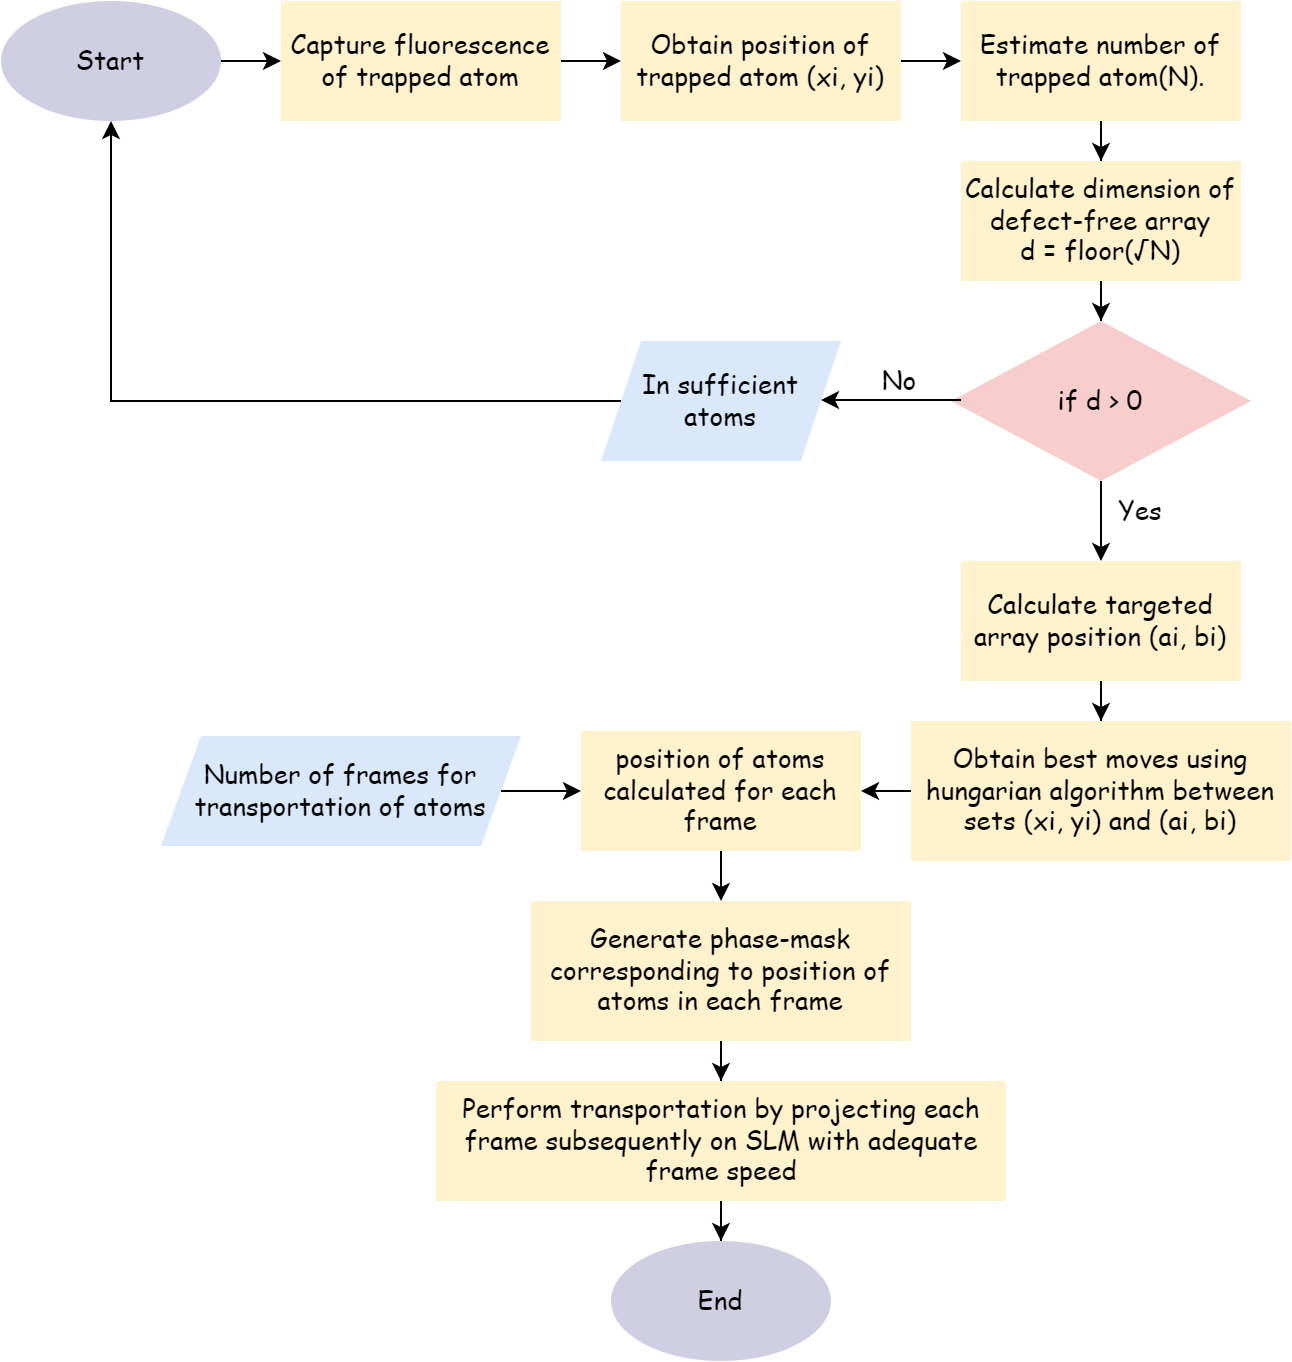
\includegraphics[width=0.9
\textwidth]{img/flowchart.png}
\caption{Flowchart of methods we have followed for the implementation of defect-free atom array}
\end{figure}

%%%%%%%%%%%%%%%%%%%%%%%%%%%%%%%%%%%%%%%%%%%%%%%%%%
%%%%%%%%%%%%%%%%%%%%%%%%%%%%%%%%%%%%%%%%%%%%%%%%%%
\section{Results and Discussion} 
\label{sec:results}
\subsection{2D array of optical traps}
We have, $|A_{source}|^2$ as shown in 5(a) while figure 5(b) shows the targeted intensity distribution ($ |A_{target}|^2 $) having a 3x3 array of tightly focused beam of optical tweezers. Using the GS algorithm, we have iteratively find the phase $\phi_{mn}$ described in equation \ref{eq:discrete_A_slm} from the random phase shown in Figure 6(a).
\begin{figure}[H]
\centering
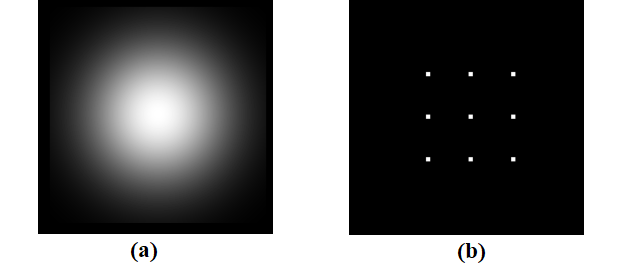
\includegraphics[width=\textwidth]{img/Target.png}
\label{fig:img_target}
\caption{(a) Source intensity distribution, (b) Target intensity distribution}
\end{figure}

\begin{figure}[H]
\label{fig:phase}
\centering
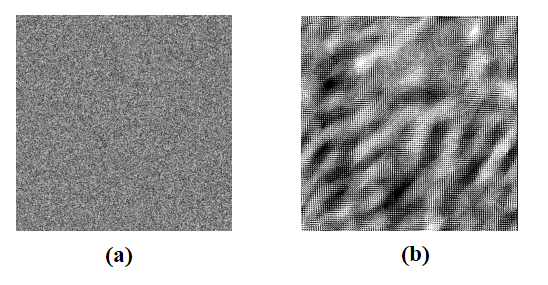
\includegraphics[width=0.91\textwidth]{img/Phase.png}
\caption{(a) Random phase, (b)Phase determined using GS Algorithm}
\end{figure}

The focal plane of the lens is imaged using a CMOS sensor which initially contains the higher diffraction order, as shown in Figure 7, so we have used the iris to select the single order and obtained the targeted intensity image. Since the SLM has a fill factor of approximately 90\%, a small portion of the reflected beam is unmodulated and appears as a bright spot in the beam's centre. We have tried to remove the unmodulated beam using the concept of the virtual lens as described in paper \cite{10.3389/fphy.2021.587112}. Nevertheless, it is not eradicated. So, we have tried to keep the array slightly far from the centre of the SLM in order to block the unmodulated beam with the iris. Figure 8(a) shows the array of tweezers imaged through the CMOS Camera, and figure 8(b) shows the intensity pattern on the screen. 

\begin{figure}[H]
\label{diff_order}
\centering
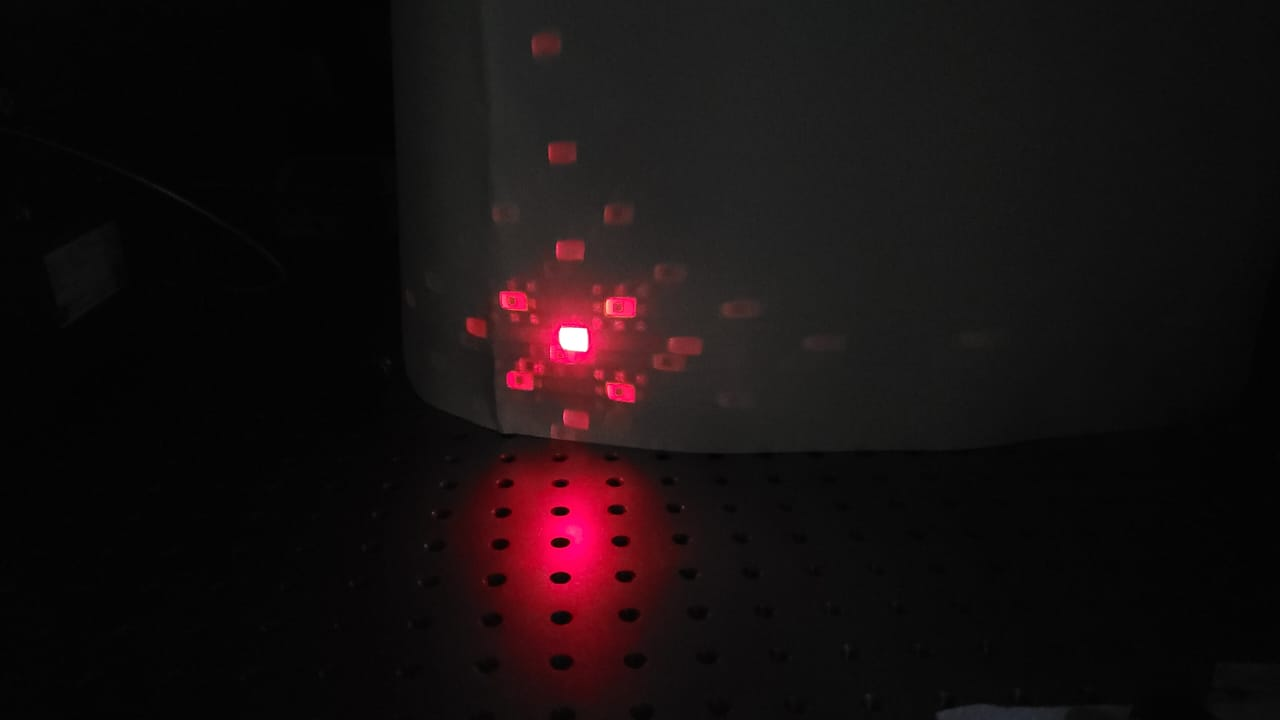
\includegraphics[width=0.9\textwidth]{img/diff.jpeg}
\caption{Diffraction Order after beam get modulated from the SLM}
\end{figure}

\vspace{1 cm}

\begin{figure}[H]
\label{img: result}
\centering
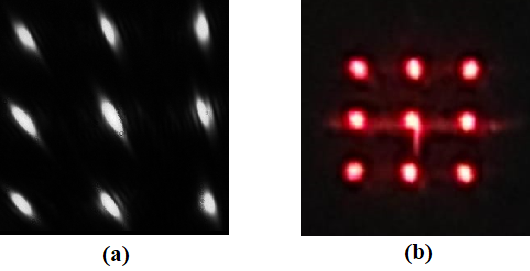
\includegraphics[width=0.9\textwidth]{img/result_img.png}
\caption{(a) Optical Tweezers imaged through CMOS Camera, (b) Optical Tweezers imaged on the screen}
\end{figure}

\vspace{0.5 cm}
We have also analysed the intensity distribution of the tweezers shown in Figure 8(a). The imaged intensity follows the gaussian pattern in both horizontal and vertical directions of traps, as depicted in figure 9. The shape is not circular, and the intensity of each trap is slightly different, maybe because we are using the circular aperture to block the diffraction orders. Imaging the focal plane of the lens without the iris gave us circular-shaped tweezers. So using a rectangular aperture for filtering instead of a circular might be beneficial.

\begin{figure}[H]
\label{img:intensity analysis}
\centering
\includegraphics[width=\textwidth]{img/20220831_4_Profile.png}
\caption{Analysis of intensity pattern of each rows and columns for the Optical Tweezers arrays of Figure 8(a)}
\end{figure}
%--------------------------------------------------------------------------------
\vspace{1.1 cm}

\subsection{Defect free array formation}
\label{subsec: defect free array}
Since the atom is not trapped yet, we have tried to simulate the trapped atom configuration by randomly generated the optical tweezers pattern. Figure 10(a) shows the randomly generated trapped configuration $(I = \{x_i, y_i\})$ with a load probability of 50 percent for each site and 10(b) shows the plot for the final configuration of atom $(T = \{a_i, b_i\})$. After implementing the Hungarian algorithm on the bipartite graph $G(I, T, E)$, we obtain the matching shown in figure 11. Experimental demonstration of optical tweezers movement is shown in figure 12 and 13.

\begin{figure}[H]
\label{fig:tweezers_plot}
\centering
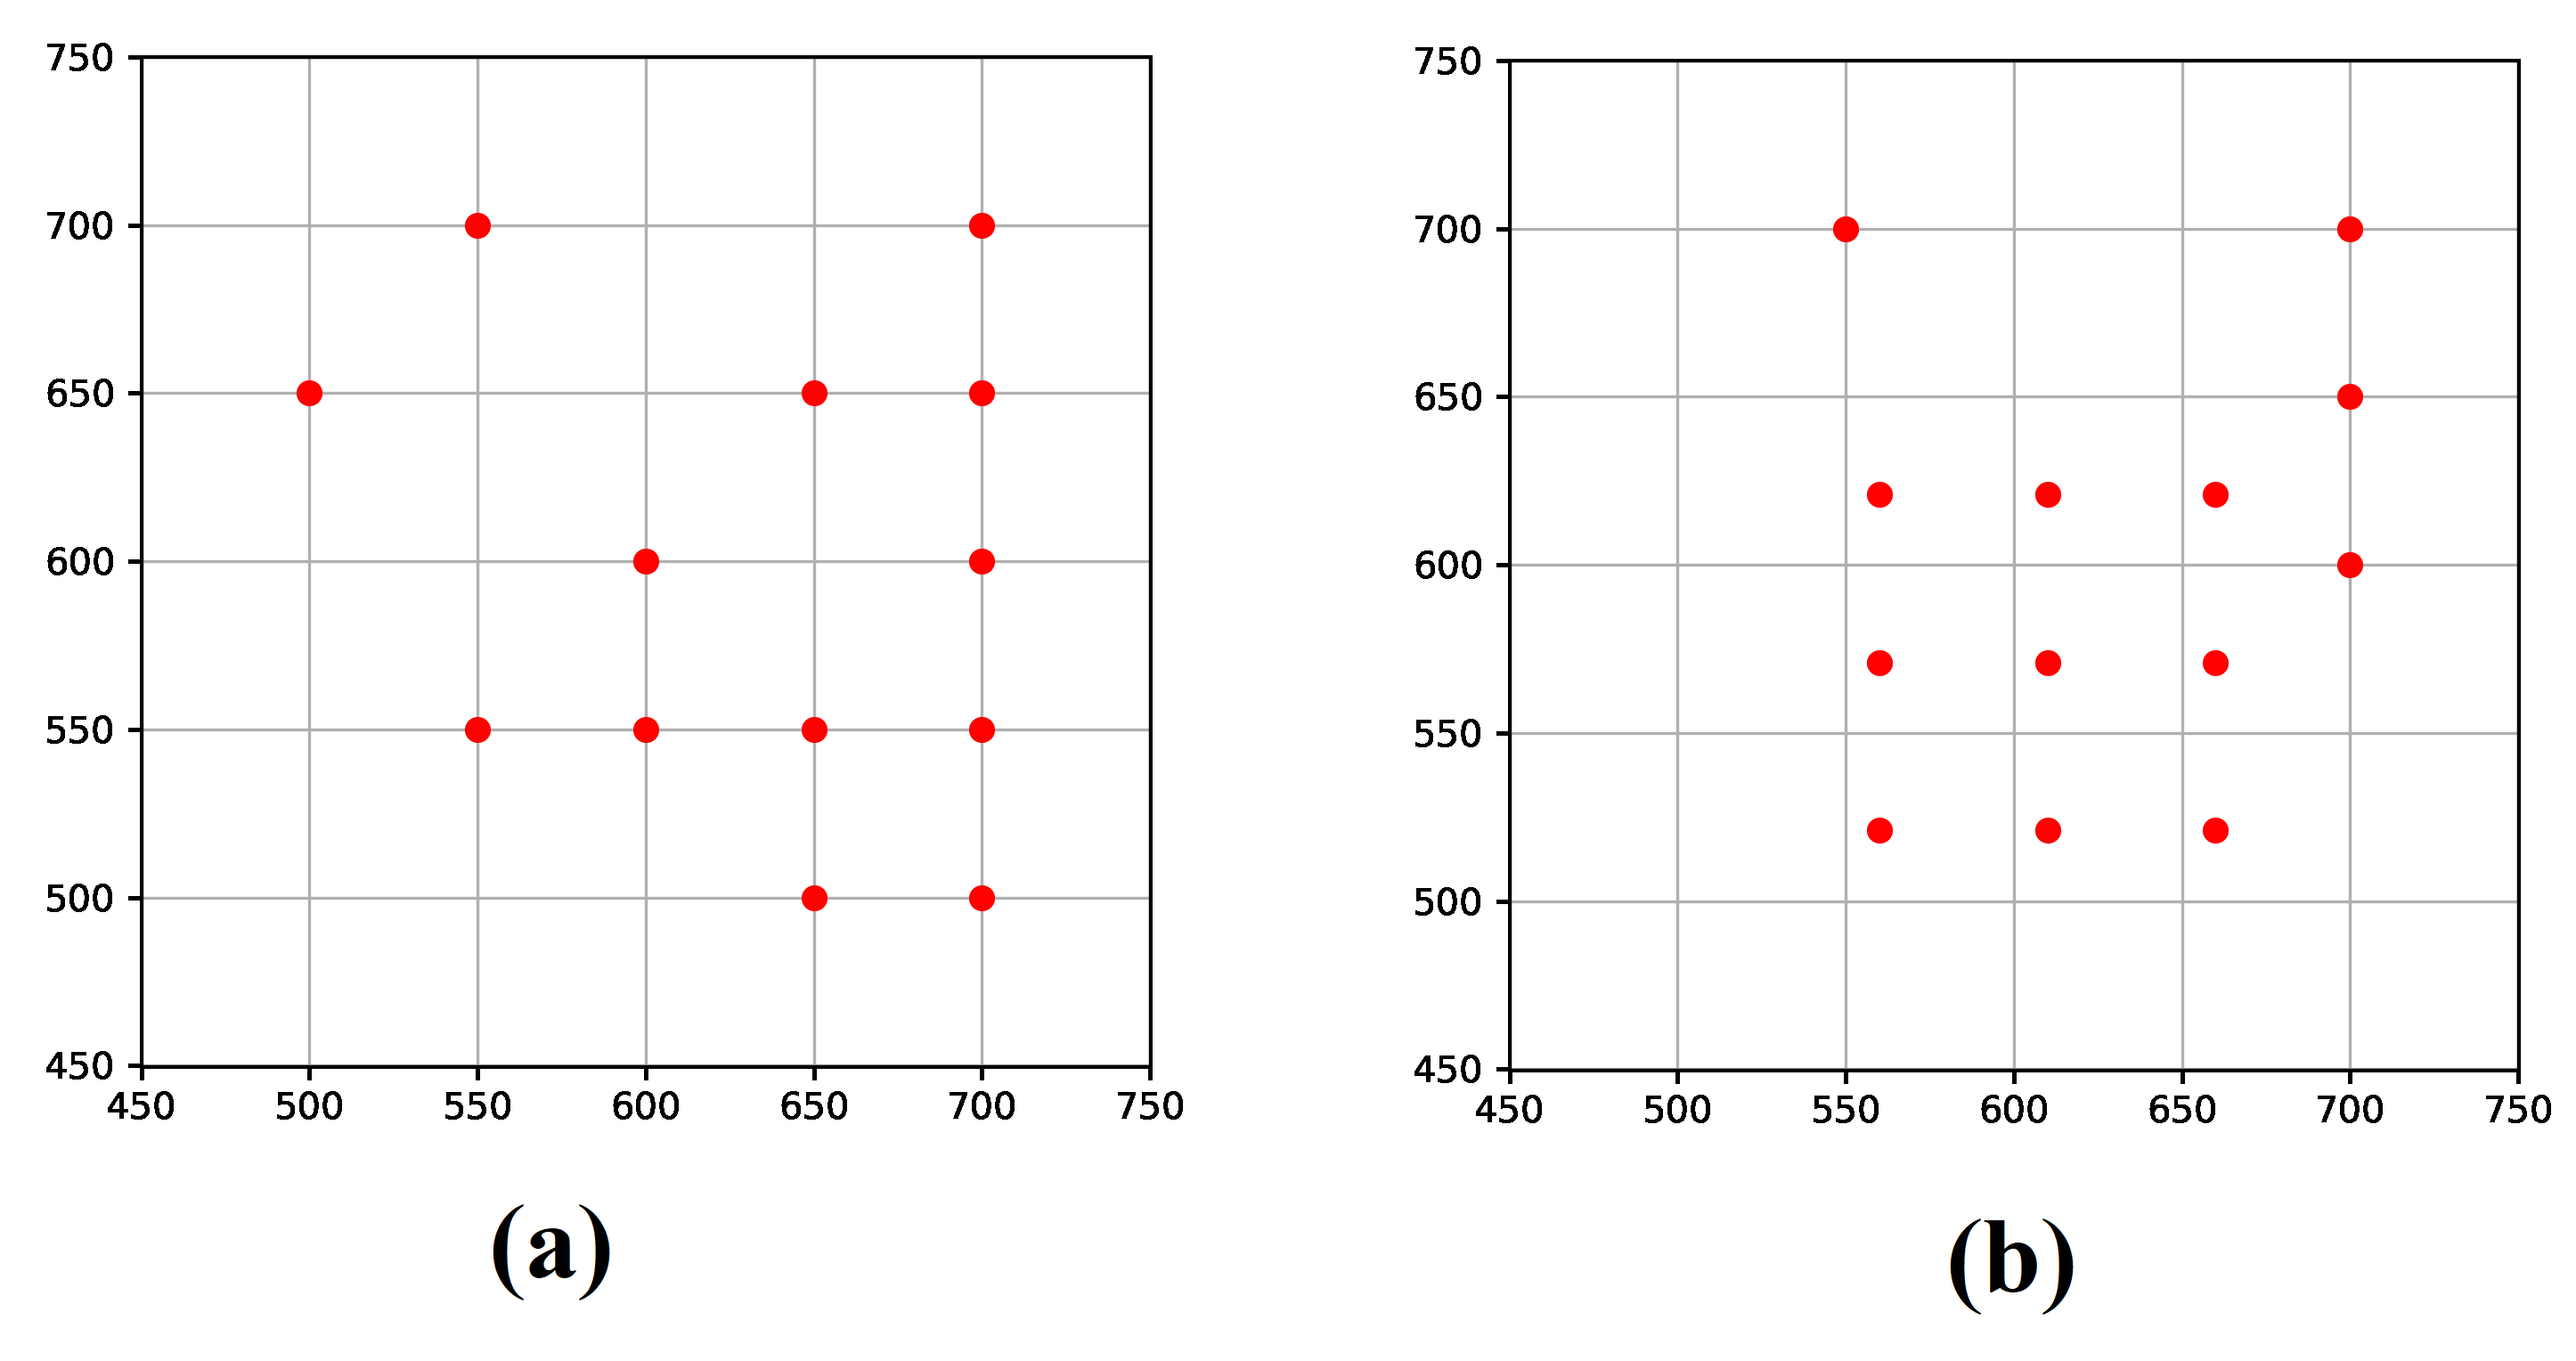
\includegraphics[width=\textwidth]{img/tweezers_plot.png}
\caption{(a) Initial configuration of trapped array, (b) Final configuration of trapped array}
\end{figure}

\begin{figure}[H]
\label{fig:combined_move}
\centering
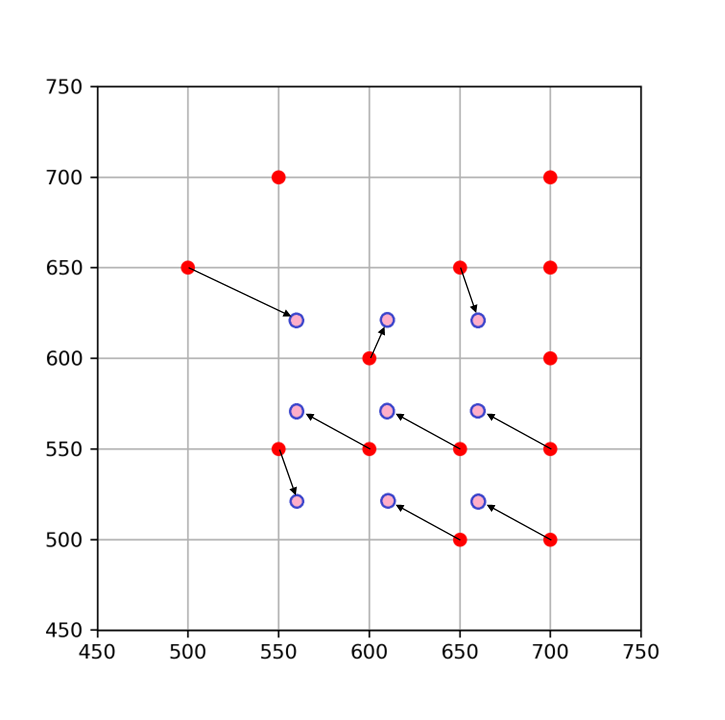
\includegraphics[width=0.65\textwidth]{img/combined_move.png}
\caption{Illustrations of the moves from an initial $5 \times 5$ array to a final $3 \times 3$ array. Simulation can be seen \href{https://drive.google.com/file/d/1JTKyHGn4GLYZHJFvZTr1iKvnrk_kMZGr/view?usp=share_link}{here}.}
\end{figure}

\vspace{0.5cm}
\begin{figure}[H]
\label{trap_slm}
\centering
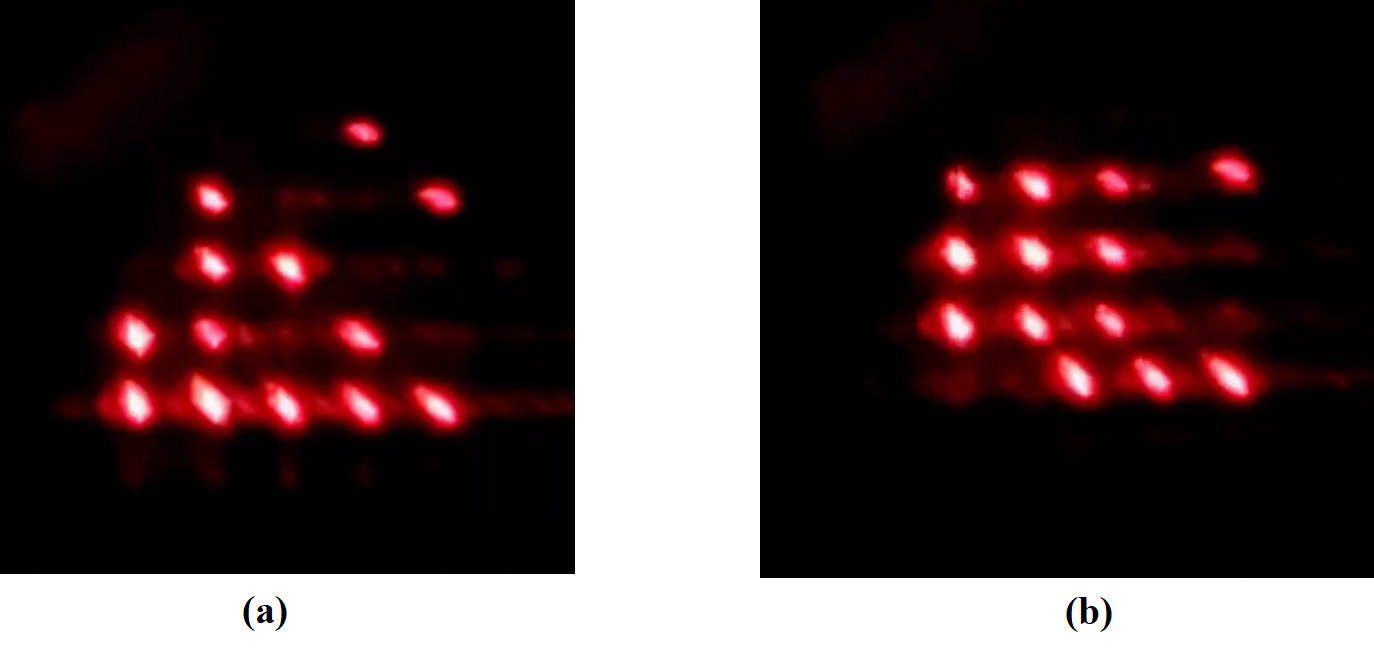
\includegraphics[width=0.9\textwidth]{img/tweezers.png}
\caption{(a) Initial configuration of trapped atom and (b) Final configuration of atom in array projected on screen}
\end{figure}

\vspace{0.8cm}
\begin{figure}[H]
\label{frames}
\centering
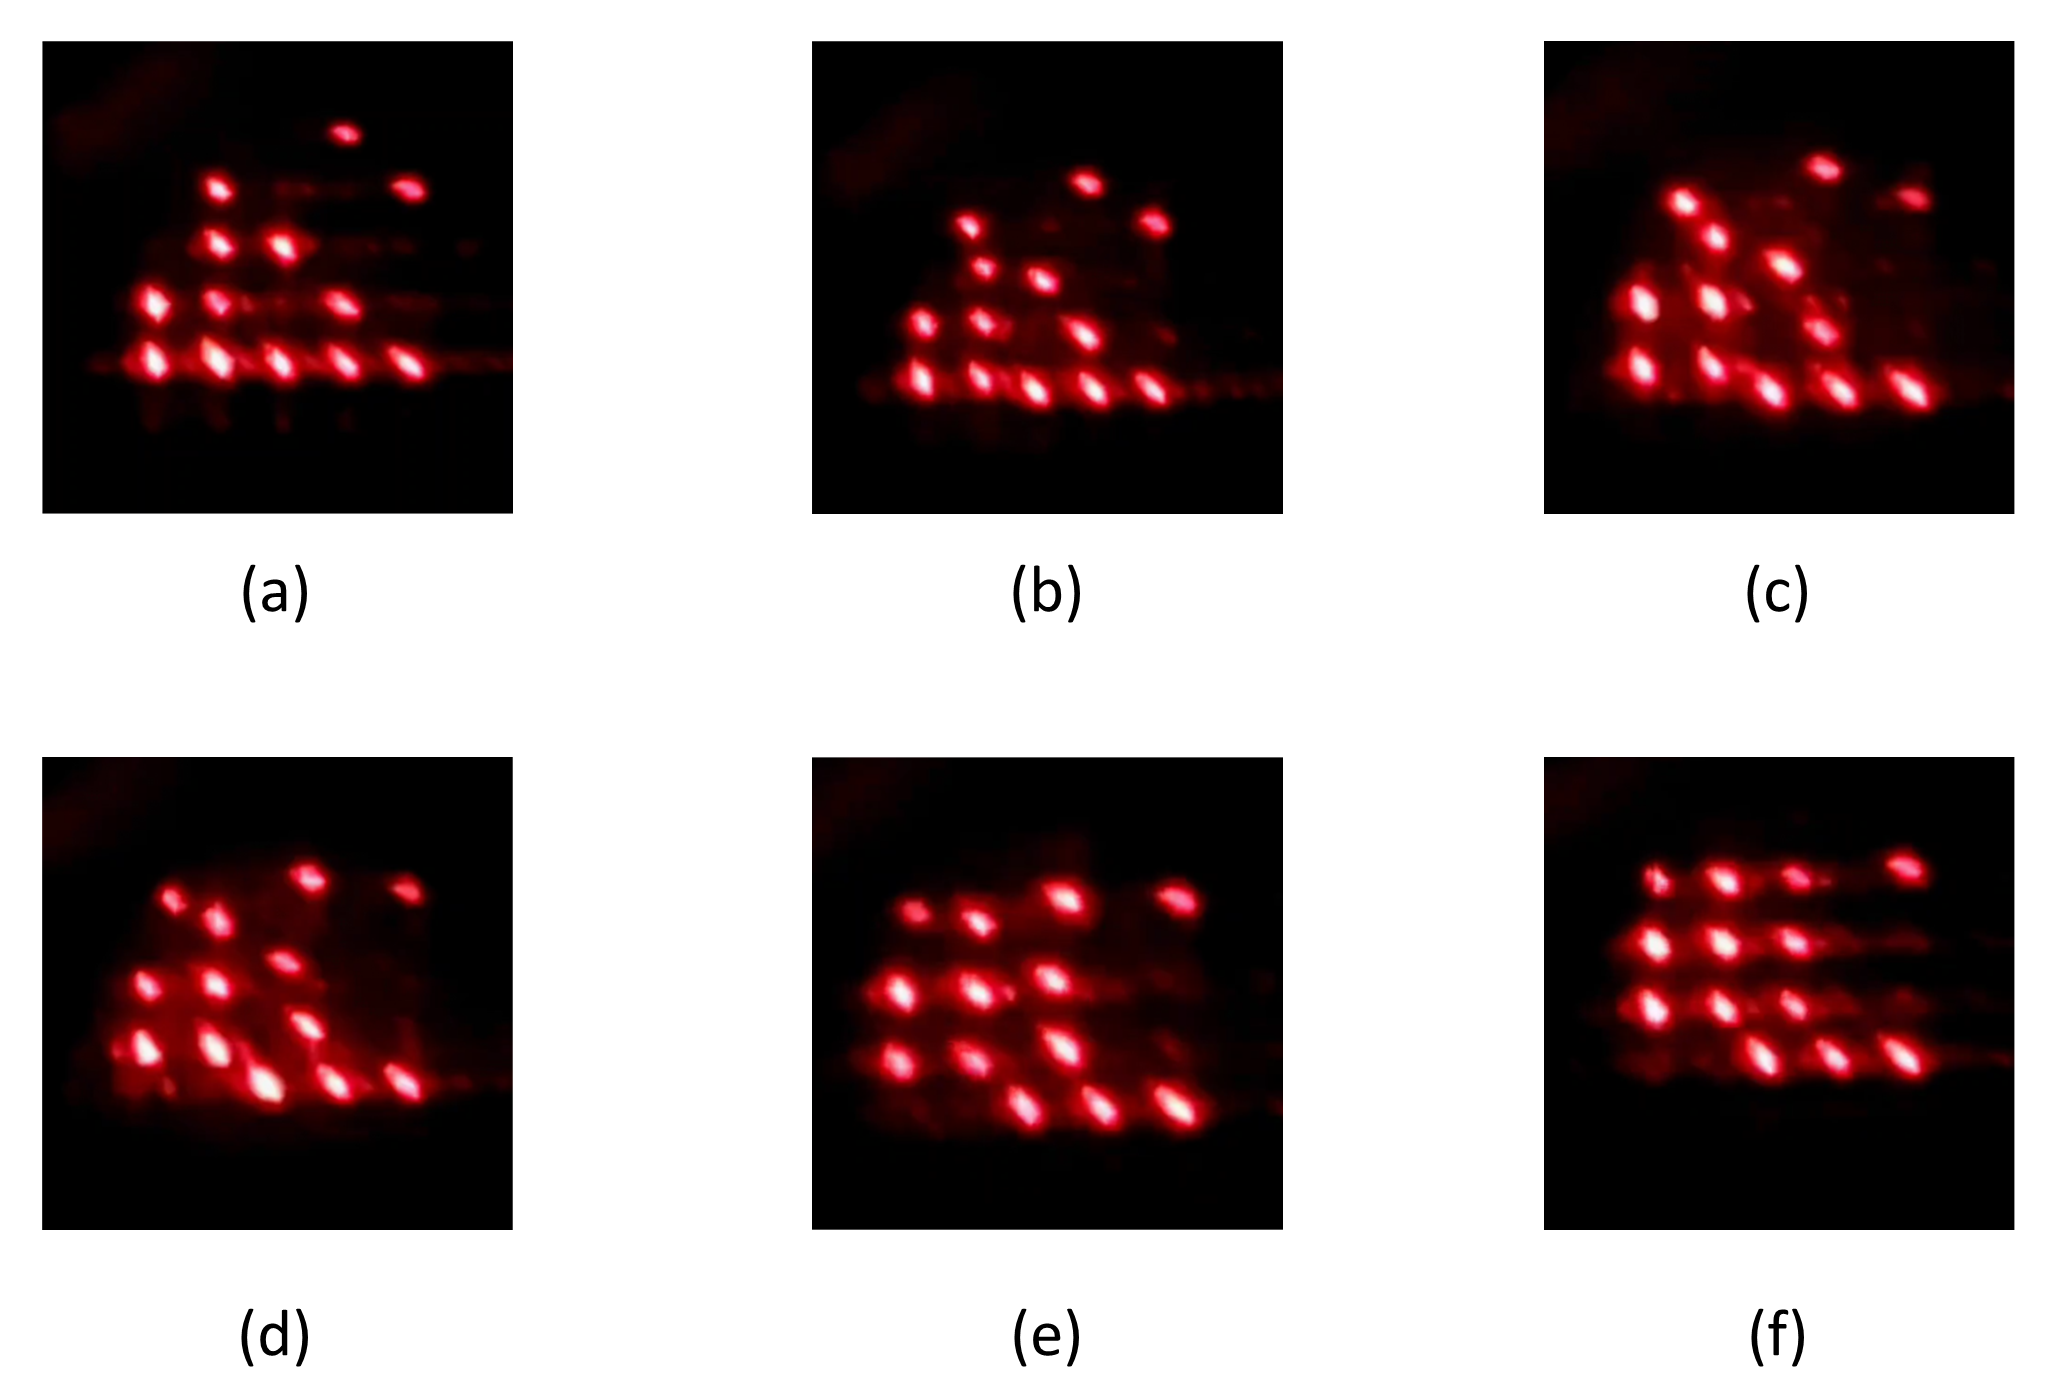
\includegraphics[width=\textwidth]{img/frame.png}
\caption{Snapshots of the frames during the movement. (a) initial frame, (b), (c), (d) and (e) are frames in between the movement and (f) is the final frame. Entire movement of optical tweezers can be seen \href{https://drive.google.com/file/d/10Ov5Z4IybwpwF9MXvInDwmm_61tb9SZ2/view?usp=sharing}{here}.}
\end{figure}

% The trapped atom configuration is generated randomly as per now.

%%%%%%%%%%%%%%%%%%%%%%%%%%%%%%%%%%%%%%%%%%%%%%%%%%%%%%%%%%%%
%%%%%%%%%%%%%%%%%%%%%%%%%%%%%%%%%%%%%%%%%%%%%%%%%%%%%%%%%%%%
\section{Conclusions}
\label{sec:Conclusion}
%%%%%%%%%%%%%%%%%%%%%%%%%%%%%%%%%%%%%%%%%%%%%%%%%%%%%%%%%%%%
%%%%%%%%%%%%%%%%%%%%%%%%%%%%%%%%%%%%%%%%%%%%%%%%%%%%%%%%%%%%
% We have demonstrated the generation of optical tweezers using the spatial light modulator.We are able to generate any 2D geometry using this method. The Gerchberg-Saxton algorithm is used to determine the optimum phase pattern for a specific trap configuration. We have determined the profile of each trap and it is found to have gaussian like structure. The need and approach to get defect-free array is discussed. We also demonstrated the movement of optical tweezers to transport the reservoir atom to vacancies.


We have demonstrated the generation of optical tweezers from arbitrary 2D geometry using the spatial light modulator scheme. The Gerchberg-Saxton algorithm is used to determine the optimal phase pattern for a specific trap configuration. We have determined the profile of each trap, and it is found to have a Gaussian-like structure. We have designed our system of trapping ~2N atoms for the requirement of N atoms in order to have a high probability of trapping N atoms, and neighbouring reservoir atoms will fill the vacant sites in the trapped array. We have obtained the optimal matching between the reservoir and vacancies using a Hungarian algorithm and experimentally demonstrated the optimal way of moving optical tweezers to transport the atom.

%%%%%%%%%%%%%%%%%%%%%%%%%%%%%%%%%%%%%%%%%%%%%%%%%%

%%%%%%%%%%%%%%%%%%%%%%%%%%%%%%%%%%%%%%%%%%%%%%%%%%%%%%%%%%%%
%%%%%%%%%%%%%%%%%%%%%%%%%%%%%%%%%%%%%%%%%%%%%%%%%%%%%%%%%%%%
\section{Future scope}
\label{sec:scope}
%%%%%%%%%%%%%%%%%%%%%%%%%%%%%%%%%%%%%%%%%%%%%%%%%%%%%%%%%%%%
%%%%%%%%%%%%%%%%%%%%%%%%%%%%%%%%%%%%%%%%%%%%%%%%%%%%%%%%%%%%
The next objective is to modify the GS algorithm to eliminate flickering in the movement of atoms using real-time feedback from the imaging camera to reduce the number of atoms destroyed during the transit process. Afterwards, we will set up the optics in accordance with the presented design and characterize the complete systems for trapping caesium atoms. In the meanwhile, work may also be done to construct a laser with a wavelength of 976 nm and characterize it.
%%%%%%%%%%%%%%%%%%%%%%%%%%%%%%%%%%%%%%%%%%%%%%%%%%


\section*{Acknowledgements}
%%%%%%%%%%%%%%%%%%%%%%%%%%%%%%%%%%%%%%%%%%%%%%%%%%%%%%%%%%%%
 I wish to express my sincere gratitude to my guide, Prof. Bodhaditya Santra, for his guidance, help, and motivation. I would like to thank him, Neha Singh and Aditya Choudhary for providing me constant support throughout the project and for believing in me.
 I am grateful to my colleagues and friends who gave me a pleasant environment to work. Last but not least, I would like to express my special thanks to my parents for their continuous motivation and support.
%%%%%%%%%%%%%%%%%%%%%%%%%%%%%%%%%%%%%%%%%%%%%%%%%%%%

%%%%%%%%%%%%%%%%%%%%%%%%%%%%%%%%%%%%%%%%%%%%%%%%%%%%%%%%%%%%
%\appendix
%%%%%%%%%%%%%%%%%%%%%%%%%%%%%%%%%%%%%%%%%%%%%%%%%%%%%%%%%%%%

%%%%%%%%%%%%%%%%%%%%%%%%%%%%%%%%%%%%%%%%%%%%%%%%%%%%%%%%%%%%
%References
% \begin{thebibliography}{99}
% %%%%%%%%%%%%%%%%%%%%%%%%%%%%%%%%%%%%%%%%%%%%%%%%%%%%%%%%%%%%
% \bibitem{Goldstein:2001} 
%   H.~Goldstein,
%   ``Classical Mechanics,'' Narosa Pub. House (2001) 702p,
%   ISBN: 9788185015538.
%   %%%%%%%%%
% \bibitem{Einstein:1916vd} 
%   A.~Einstein,
%   ``The Foundation of the General Theory of Relativity,''
%   Annalen Phys.\  {\bf 49}, no. 7, 769 (1916).
% %%%%%%%%%
% \bibitem{Einstein:1935tc} 
%   A.~Einstein and N.~Rosen,
%   ``The Particle Problem in the General Theory of Relativity,''
%   Phys.\ Rev.\  {\bf 48}, 73 (1935).
% %%%%%%%%%  
%   \bibitem{Dirac:1948um} 
%   P.~A.~M.~Dirac,
%   ``The Theory of magnetic poles,''
%   Phys.\ Rev.\  {\bf 74}, 817 (1948).
% %%%%%%%%% 
%   \bibitem{iitd:web} 
%   See \href{http://www.sharelatex.com}{IIT Delhi Physics}
% \end{thebibliography}
% \include{ref.tex}

\bibliographystyle{unsrt}
\bibliography{ref.bib}
% \newpage
% \begin{figure}[H]
% \centering
% 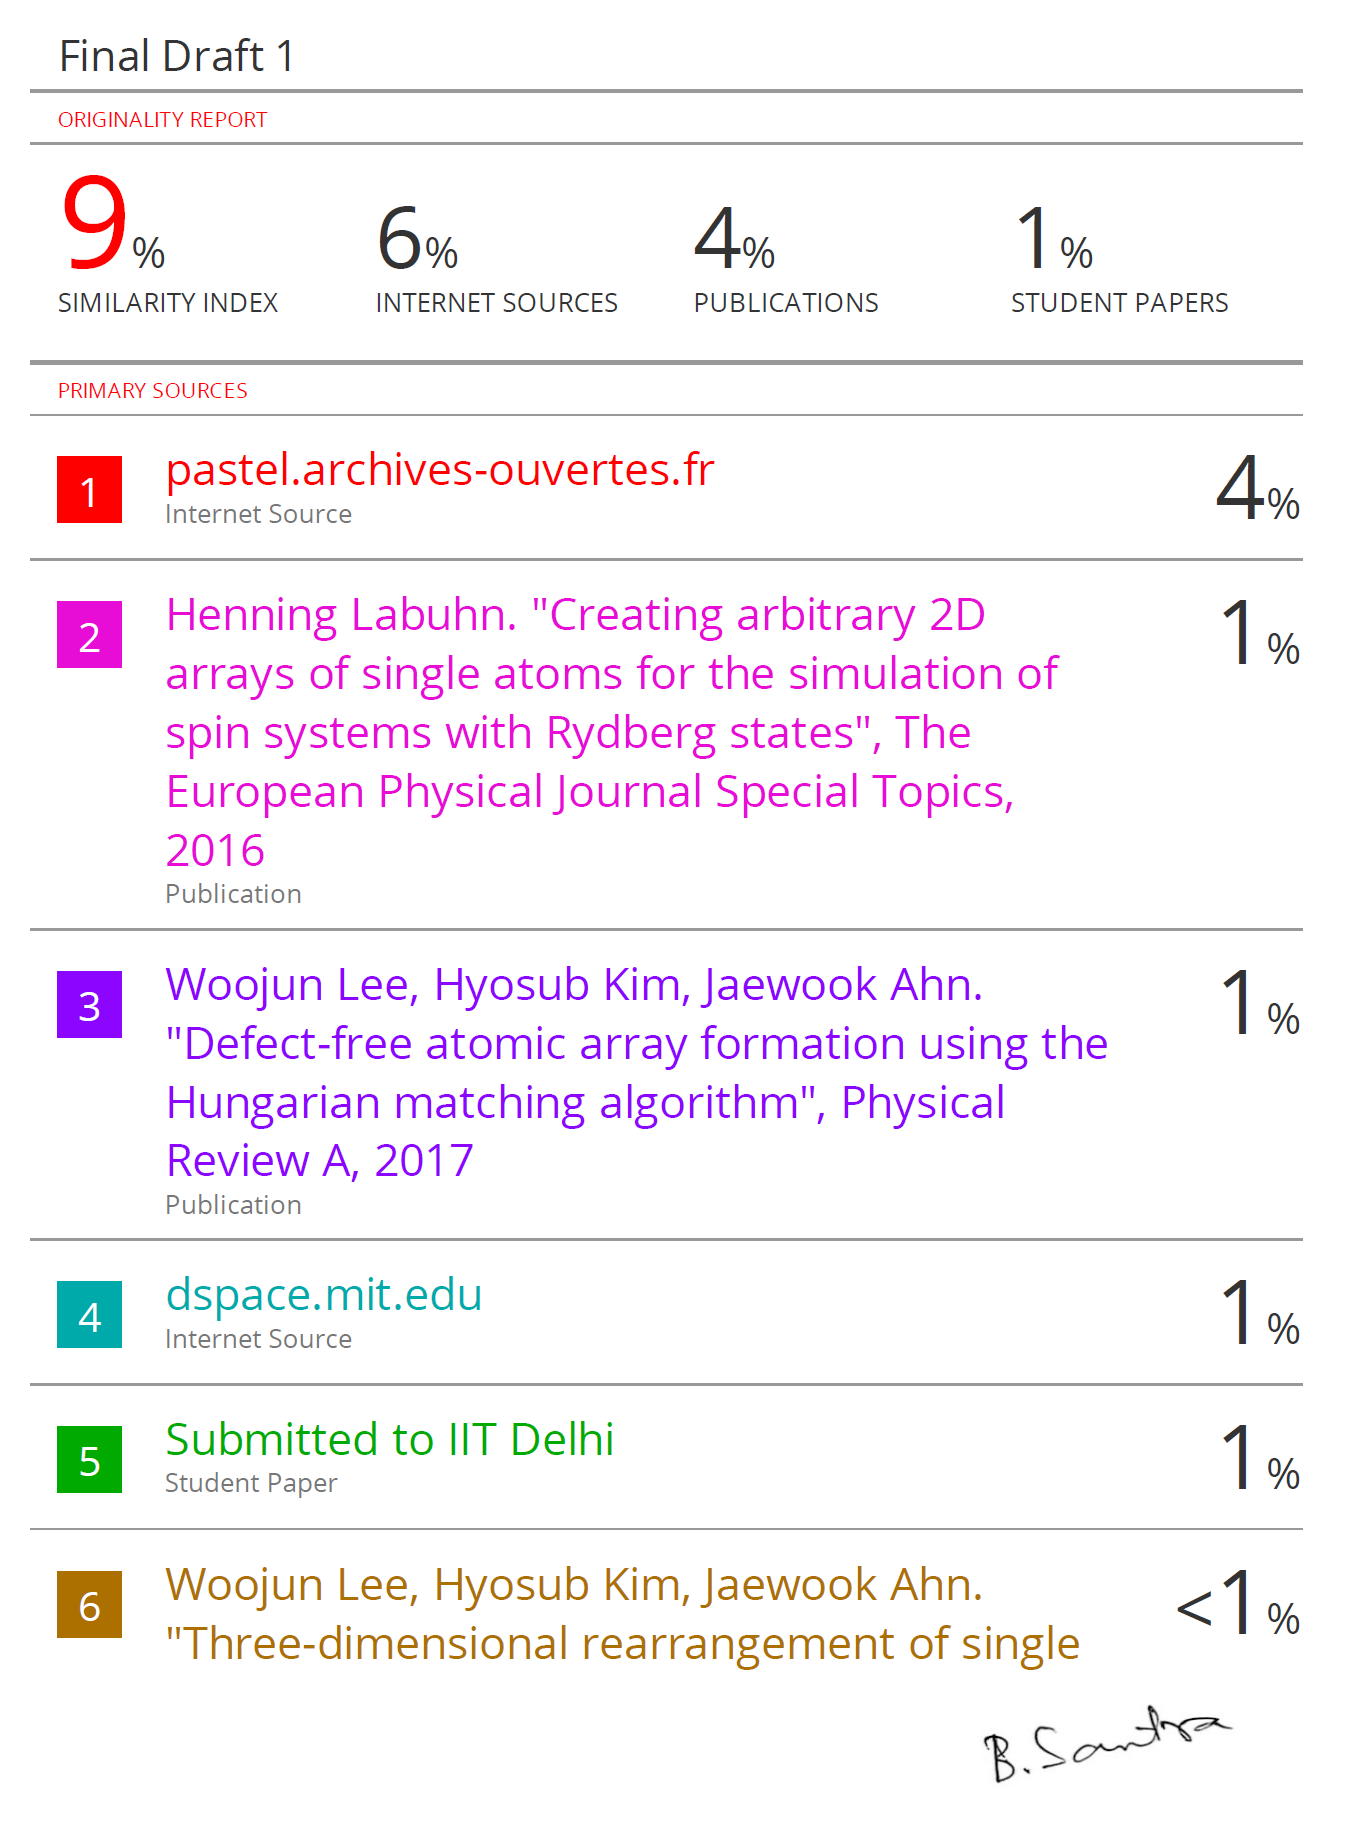
\includegraphics[width=\textwidth]{img/turnitin report.png}
% \end{figure}
%%%%%%%%%%%%%%%%%%%%%%%%%%%%%%%%%%%%%%%%%%%%%%%%%%%%%%%%%%%%
\end{document}
